\textbf{Patrocinadores que solo esten patrocinando a una disciplina.}\vspace{.3cm}

\begin{center}
	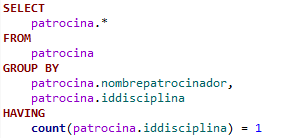
\includegraphics[width=1.05\textwidth]{resources/consulta5.png}
\end{center} 

\textbf{Explicación:} \\
Aquí seleccionamos los datos de la tabla patrocina, luego agrupamos por nombrepatrocinador e iddisciplina para organizar la información de patrocinadores y disciplinas. Con el uso de having count(patrocina.iddisciplina) = 1, filtramos los patrocinadores que solo tienen una entrada en la tabla patrocina, lo cual significa que están patrocinando exclusivamente una disciplina.\vspace{.3cm}

\textbf{Resultado:}
\begin{center}
	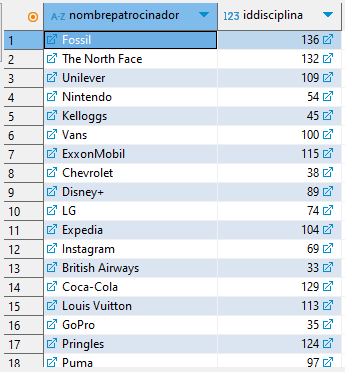
\includegraphics[width=1.05\textwidth]{resources/resultados/r5.png}
\end{center} 